% This file makes a printable version of the blueprint
% It should include all the \usepackage needed for the pdf version.
% The template version assume you want to use a modern TeX compiler
% such as xeLaTeX or luaLaTeX including support for unicode
% and Latin Modern Math font with standard bugfixes applied.
% It also uses expl3 in order to support macros related to the dependency graph.
% It also includes standard AMS packages (and their improved version
% mathtools) as well as support for links with a sober decoration
% (no ugly rectangles around links).
% It is otherwise a very minimal preamble (you should probably at least
% add cleveref and tikz-cd).

\documentclass[a4paper]{report}

\usepackage{geometry}

\usepackage{expl3}

\usepackage{amssymb, amsthm, mathtools}
\usepackage[unicode,colorlinks=true,linkcolor=blue,urlcolor=magenta, citecolor=blue]{hyperref}

\usepackage[warnings-off={mathtools-colon,mathtools-overbracket}]{unicode-math}
%  For enumerating root system axioms
\usepackage{enumitem}

% In this file you should put all LaTeX macros and settings to be used both by
% the pdf version and the web version.
% This should be most of your macros.

% The theorem-like environments defined below are those that appear by default
% in the dependency graph. See the README of leanblueprint if you need help to
% customize this. 
% The configuration below use the theorem counter for all those environments
% (this is what the [theorem] arguments mean) and never resets it.
% If you want for instance to number them within chapters then you can add
% [chapter] at the end of the next line.
\newtheorem{theorem}{Theorem}
\newtheorem{proposition}[theorem]{Proposition}
\newtheorem{lemma}[theorem]{Lemma}
\newtheorem{corollary}[theorem]{Corollary}

\newtheorem{definition}[theorem]{Definition}
\newenvironment{nameddefinition}[1]{%
    \par\noindent\textbf{Definition (#1).}\ \ignorespaces%
}{%
    \par\medskip%
}

\newenvironment{namedtheorem}[1]{%
    \par\noindent\textbf{Theorem (#1).}\ \ignorespaces%
}{%
    \par\medskip%
}

\newtheorem{example}[theorem]{Example}
% This file makes a printable version of the blueprint
% It should include all the \usepackage needed for the pdf version.
% The template version assume you want to use a modern TeX compiler
% such as xeLaTeX or luaLaTeX including support for unicode
% and Latin Modern Math font with standard bugfixes applied.
% It also uses expl3 in order to support macros related to the dependency graph.
% It also includes standard AMS packages (and their improved version
% mathtools) as well as support for links with a sober decoration
% (no ugly rectangles around links).
% It is otherwise a very minimal preamble (you should probably at least
% add cleveref and tikz-cd).

\documentclass[a4paper]{report}

\usepackage{amssymb, amsthm, mathtools}
\usepackage[unicode,colorlinks=true,linkcolor=blue,urlcolor=magenta, citecolor=blue]{hyperref}
\usepackage{preamble}

% In this file you should put all LaTeX macros and settings to be used both by
% the pdf version and the web version.
% This should be most of your macros.

% The theorem-like environments defined below are those that appear by default
% in the dependency graph. See the README of leanblueprint if you need help to
% customize this. 
% The configuration below use the theorem counter for all those environments
% (this is what the [theorem] arguments mean) and never resets it.
% If you want for instance to number them within chapters then you can add
% [chapter] at the end of the next line.
\newtheorem{theorem}{Theorem}
\newtheorem{proposition}[theorem]{Proposition}
\newtheorem{lemma}[theorem]{Lemma}
\newtheorem{corollary}[theorem]{Corollary}

\newtheorem{definition}[theorem]{Definition}
\newenvironment{nameddefinition}[1]{%
    \par\noindent\textbf{Definition (#1).}\ \ignorespaces%
}{%
    \par\medskip%
}

\newenvironment{namedtheorem}[1]{%
    \par\noindent\textbf{Theorem (#1).}\ \ignorespaces%
}{%
    \par\medskip%
}

\newtheorem{example}[theorem]{Example}
% This file makes a printable version of the blueprint
% It should include all the \usepackage needed for the pdf version.
% The template version assume you want to use a modern TeX compiler
% such as xeLaTeX or luaLaTeX including support for unicode
% and Latin Modern Math font with standard bugfixes applied.
% It also uses expl3 in order to support macros related to the dependency graph.
% It also includes standard AMS packages (and their improved version
% mathtools) as well as support for links with a sober decoration
% (no ugly rectangles around links).
% It is otherwise a very minimal preamble (you should probably at least
% add cleveref and tikz-cd).

\documentclass[a4paper]{report}

\usepackage{amssymb, amsthm, mathtools}
\usepackage[unicode,colorlinks=true,linkcolor=blue,urlcolor=magenta, citecolor=blue]{hyperref}
\usepackage{preamble}

% In this file you should put all LaTeX macros and settings to be used both by
% the pdf version and the web version.
% This should be most of your macros.

% The theorem-like environments defined below are those that appear by default
% in the dependency graph. See the README of leanblueprint if you need help to
% customize this. 
% The configuration below use the theorem counter for all those environments
% (this is what the [theorem] arguments mean) and never resets it.
% If you want for instance to number them within chapters then you can add
% [chapter] at the end of the next line.
\newtheorem{theorem}{Theorem}
\newtheorem{proposition}[theorem]{Proposition}
\newtheorem{lemma}[theorem]{Lemma}
\newtheorem{corollary}[theorem]{Corollary}

\newtheorem{definition}[theorem]{Definition}
\newenvironment{nameddefinition}[1]{%
    \par\noindent\textbf{Definition (#1).}\ \ignorespaces%
}{%
    \par\medskip%
}

\newenvironment{namedtheorem}[1]{%
    \par\noindent\textbf{Theorem (#1).}\ \ignorespaces%
}{%
    \par\medskip%
}

\newtheorem{example}[theorem]{Example}
% This file makes a printable version of the blueprint
% It should include all the \usepackage needed for the pdf version.
% The template version assume you want to use a modern TeX compiler
% such as xeLaTeX or luaLaTeX including support for unicode
% and Latin Modern Math font with standard bugfixes applied.
% It also uses expl3 in order to support macros related to the dependency graph.
% It also includes standard AMS packages (and their improved version
% mathtools) as well as support for links with a sober decoration
% (no ugly rectangles around links).
% It is otherwise a very minimal preamble (you should probably at least
% add cleveref and tikz-cd).

\documentclass[a4paper]{report}

\usepackage{amssymb, amsthm, mathtools}
\usepackage[unicode,colorlinks=true,linkcolor=blue,urlcolor=magenta, citecolor=blue]{hyperref}
\usepackage{preamble}

\input{macros/common}
\input{macros/print}

\title{Classification of Root Systems}
\author{Shaheer Ziya}

\begin{document}
\maketitle
\input{content}
\end{document}

\title{Classification of Root Systems}
\author{Shaheer Ziya}

\begin{document}
\maketitle
% In this file you should put the actual content of the blueprint.
% It will be used both by the web and the print version.
% It should *not* include the \begin{document}
%
% If you want to split the blueprint content into several files then
% the current file can be a simple sequence of \input. Otherwise It
% can start with a \section or \chapter for instance.


\input{Chapters/chapter_1.tex}
\end{document}

\title{Classification of Root Systems}
\author{Shaheer Ziya}

\begin{document}
\maketitle
% In this file you should put the actual content of the blueprint.
% It will be used both by the web and the print version.
% It should *not* include the \begin{document}
%
% If you want to split the blueprint content into several files then
% the current file can be a simple sequence of \input. Otherwise It
% can start with a \section or \chapter for instance.


\chapter{Root Systems}
\section{Defining Root Systems}

\begin{nameddefinition}{Root System}
    Let $E$ be a finite-dimensional Euclidean space with an inner product $\langle \cdot, \cdot \rangle$. \newline
    
    A \textbf{root system} in $E$ is a tuple (E, $\Phi$), where $\Phi$ is a finite, non-empty set of non-zero vectors (called
    \textbf{roots}) satisfying the following properties:
    
    \begin{enumerate}[label=(R{\arabic*})]
        \item $\Phi$ spans $E$.
        \item For every root $\alpha \in \Phi$, the set $\Phi$ is closed under reflection through the hyperplane orthogonal to $\alpha$.
        That is, for any two roots $\alpha, \beta \in \Phi$, the set $\Phi$ contains the element
        \begin{equation*}
            \sigma_\alpha(\beta) = \beta - 2 \ \text{proj}_{\alpha}(\beta).
        \end{equation*}
        where $\text{proj}_{\alpha}(\beta)$ is the projection of $\beta$ on $\alpha$ as shown below.
        \begin{equation*}
            \text{proj}_{\alpha}(\beta) := \frac{ \langle \alpha, \beta \rangle}{\langle \alpha, \alpha \rangle} \alpha
        \end{equation*}
    \end{enumerate}

    The \textbf{rank} of the root system is the dimension of the Euclidean space $E$.
\end{nameddefinition}

For convenience and in contexts where the inner product space is clear, the root system is often referred to simply as $\Phi$.

\begin{example}
    $R_0 = \{\pm \alpha\}$, where $\alpha$ is any fixed non-zero real number, constitutes a root system in $\mathbb{R}$.
\end{example}

\begin{nameddefinition}{Reduced Root System}
    If a root system satisfies the condition that the only multiples of a root, $\alpha$, that are in the root system
    are $\pm \alpha$, then the root system is said to be \textbf{reduced}.
\end{nameddefinition}

\begin{nameddefinition}{Crystallographic Root System}
    If a root system satisfies the integrality condition below, then it is said to be \textbf{crystallographic}.
    \begin{equation*}
        \langle \langle \beta, \alpha \rangle \rangle = 2 \frac{ \langle \alpha, \beta \rangle}{\langle \alpha, \alpha \rangle}
        \in \mathbb{Z} \ \text{for all} \ \alpha, \beta \in \Phi
    \end{equation*}
\end{nameddefinition}

Throughout this text, denote $e_i$ as the $i$-th standard basis vector in $\mathbb{R}^n$.
Then, in combinations such as $\pm e_i \pm e_j$, the signs may be chosen independently.

\begin{example}
    The set $R_1$, shown below, is a root system in $\mathbb{R}^2$ that is neither reduced nor crystallographic.
    \begin{equation*}
        R_1 = \{
            \pm e_1, (\pm \frac{\sqrt{3}}{2}, \pm \frac{1}{2}), (\pm \sqrt{3}, \pm 1) 
        \} 
    \end{equation*}
    $R_1$ spans $\mathbb{R}^2$ and is closed under reflection through the hyperplane orthogonal to any root,
    hence it is a root system.
    
    However, is is not a \textbf{reduced} root system since a scalar multiple of an element in $R_1$,
    namely $2 \cdot (\pm \frac{1}{2}, \pm \frac{\sqrt{3}}{2})$, is contained in $R_1$ itself. 
    It is also not a \textbf{crystallographic} root system because 
    $\langle \langle e_1, (\pm \frac{\sqrt{3}}{2}, \pm \frac{1}{2}) \rangle \rangle = \frac{\sqrt{3}}{2} \notin \mathbb{Z}$.
\end{example}

\begin{example}
    If we remove the redundant multiple in $R_1$ above, we obtain a reduced, non-crystallographic root system $R_2$.
    \begin{equation*}
        R_2 = \{
            \pm e_1, (\pm \frac{\sqrt{3}}{2}, \pm \frac{1}{2})
        \} 
    \end{equation*}
\end{example}

One can also construct examples of non-reduced crystallographic root systems. Consider the following example,

\begin{example}
    The set $R_3$ is a root system in $\mathbb{R}^2$ that is crystallographic but not reduced.
    
    \begin{equation*}
        R_3 = \{
            \pm e_1, \pm e_2, \pm 2 e_1
        \} 
    \end{equation*}
    $R_3$ spans $\mathbb{R}^2$ and is closed under reflection through the hyperplane orthogonal to any root,
    hence it is a root system.
    It is a \textbf{crystallographic} root system because
    $\langle \langle k e_1, e_2 \rangle \rangle = 0$ and $\langle \langle k e_1, k' e_1 \rangle \rangle = kk' \in \mathbb{Z}$,
    where $k,k \in \{\pm 1, \pm 2\}$.
    However, is is not a \textbf{reduced} root system since $2 e_1 \in R_3$.
\end{example}


\begin{example}
    The set $R_4$ is a root system in $\mathbb{R}^2$ that is reduced and crystallographic.
    \begin{equation*}
        R_4 = \{
            \pm e_1, \pm e_2
            \} 
    \end{equation*}
\end{example}

Therefore, we see that a root system may be reduced, crystallographic, both, or neither. \newline

It should be noted that for crystallographic root systems, the integrality condition implies the second condtion (R2)
in root systems since $\sigma_{\alpha}(\alpha) = -\alpha$.
The integrality condition can be interpretted geometerically as follows--the projection of $\beta$ on $\alpha$ is
an integer or half-integer multiple of $\alpha$ since,

\begin{equation*}
    \text{proj}_{\alpha}(\beta) = \frac{1}{2} \langle \langle \beta, \alpha \rangle \rangle \alpha
\end{equation*}

In fact, this is the most restrictive condition since,
\begin{equation*}
    \langle \langle \beta, \alpha \rangle \rangle 
    =  2 \frac{ \langle \alpha, \beta \rangle}{\langle \alpha, \alpha \rangle}
    = 2 \frac{\|\beta\| \|\alpha\| \cos\theta }{\|\alpha\|^2}
    = 2 \frac{\|\beta\|}{\|\alpha\|} \in \mathbb{Z},
\end{equation*}
where $\theta$ is the angle between $\alpha$ and $\beta$.

Furthermore, since $\langle \langle \beta, \alpha \rangle \rangle$ and $\langle \langle \alpha, \beta \rangle \rangle$
must be integers,

\begin{equation*}
    \langle \langle \beta, \alpha \rangle \rangle \cdot \langle \langle \alpha, \beta \rangle \rangle = 4 \cos^2 \theta \in \mathbb{Z}
\end{equation*}

We restate this result as the following lemma.
\begin{lemma}
    For any two roots $\alpha, \beta \in \Phi$, the product
    $\langle \langle \beta, \alpha \rangle \rangle \cdot \langle \langle \alpha, \beta \rangle \rangle$ is an integer.
    More precisely, $4 \cos^2 \theta \in \{ 0, 1, 2, 3, 4 \}.$
    If $4 \cos^2 \theta = 4$, then $\theta = 0$ or $\pi$ and $\beta = \pm \alpha$ which is exactly condition $(R2)$ for a root system.
\end{lemma}

The possible values for $4 \cos^2 \theta$ and the corresponding angles between the roots are displayed in the table below.

\begin{table}[h]
\label{table:enum}
\begin{center}
\begin{tabular}{|| c  c  c  c  c ||}
    \hline $4\cos^2\theta$
&   $\langle \langle \alpha, \beta \rangle \rangle$
&   $\langle \langle \beta, \alpha \rangle \rangle$
&   $\|\alpha\| / \|\beta\|$
&   $\theta$ \\ \hline \hline
    0 & 0 & 0 & N/A & $\pi/2$ \\ \hline
    
    1 & 1 & 1 & 1 & $\pi/3$ \\
      & -1 & -1 & 1 & $2\pi/3$ \\ \hline
    
    2 & 1 & 2 & $\sqrt{2}$ & $\pi/4$  \\
      & -1 & -2 & $\sqrt{2}$ & $3\pi/4$ \\ \hline
    
    3 & 1 & 3 & $\sqrt{3}$ & $\pi/6$ \\
      &-1 & -3 & $\sqrt{3}$ & $5\pi/6$ \\ \hline
\end{tabular}
\end{center}
\caption{The possible angles between roots where, without loss of generality,
the root $\alpha$ is no longer than the root $\beta$ under the induced norm in $E$.
A computation also reveals that $|\langle \beta, \alpha \rangle| \geq |\langle \alpha, \beta \rangle|$.}
\end{table}

Since we aim to classify all root systems, upto isomorhism, it is important to understand when two root systems are
isomorphic. \newline

\begin{nameddefinition}{Root System Isomorphism}
    Two root systems $(E, \Phi)$ and $(F,\Psi)$ are said to be isomorphic if there exists a linear isomorphism
    $\varphi: E \to F$ such that $\varphi(\Phi) = \Psi$
    and preserves the number $\langle \langle x, y \rangle \rangle$ for each pair of roots.
\end{nameddefinition}

\begin{example}
    The root systems $R = \{ \pm e_1, \pm e_2 \} $ and $R' = \{ \pm e_1 \pm e_2 \}$ are isomorphic.
\end{example}

\begin{example}
    The root systems
    $S = \{ \pm e_1, \pm e_2, \pm e_1 \pm e_2 \} $ and
    $S' = \{ \pm e_1, (\pm \frac{\sqrt{3}}{2}, \pm \frac{1}{2}) \}$ are not isomorphic.
\end{example}

Finally, we wish to exclude root systems that can be constructed from direct sums of smaller root systems.
This motivates the following definition. \newline

\begin{nameddefinition}{Decomposable Root System}
    A Root System $\Phi$ is said to be \textbf{decomposable} if there is a proper decomposition
    $\Phi = \Phi_1 \cup \Phi_2$ such that $\Phi_1$ and $\Phi_2$ are root systems in $E$ and $\Phi_1 \perp \Phi_2$ (i.e. 
    $\forall \alpha_1 \in \Phi_1 , \forall \alpha_2 \in \Phi_2,  \langle \alpha_1, \alpha_2 \rangle = 0$). \newline 

    Otherwise, $\Phi$ is said to be \textbf{indecomposable}. 
    Often, in literature, such root systems are also called \textbf{irreducible}.
    We adopt the term indecomposable to avoid confusion with the notion of reduced root systems.
\end{nameddefinition}

\begin{example}
    The root system $R_4 = \{ \pm e_1, \pm e_2 \}$ is an indecomposable, reduced, crystallographic root system.
\end{example}

\begin{example}
    The root system $R_5 = \{ \pm e_1, \pm e_2 \} \cup \{ \pm 2 e_1 \}$ is a decomposable root system.
\end{example}

This report concerns itself primarily with reduced, crystallographic root systems, simply referred to as root systems henceforth,
unless otherwise specified.

\footnote{
    The provided definition differs from the more general definition stated in Lean 4's MathLib.
    In Lean 4, root systems are defined over modules instead of Euclidean spaces among other minor differences.
    As such, when neccessary the proofs in Lean 4 restrict the more general definition to our definition.
    Of note, root systems in Lean 4 are assumed to be reduced, crystallographic root systems.} \newline

    \section{Classifying Root Systems of Small Rank}

% Classification of Rank 1 Root Systems
\begin{namedtheorem}{Classification of Rank 1 Root Systems}
    The only indecomposable, reduced, crystallographic root systems of rank 1 (upto isomorhism) is $A_1 = \{ \pm \alpha \}$ [See Figure 1.1], where $\alpha$ is any fixed non-zero real number.
\end{namedtheorem}

\begin{proof}
    Let $\Phi$ be a reduced, crystallographic root system of rank 1.
    Let $\alpha \in \Phi$ be a non-zero root.
    Since $\Phi$ is reduced, the only multiples of $\alpha$ in $\Phi$ are $\pm \alpha$.
    Therefore, $\Phi = \{ \pm \alpha \}$.
    Clearly, if the root system depends on $\alpha$ where $\Phi_{\alpha} = \{ \pm \alpha \}$,
    then for any non-zero $\alpha_1, \alpha_2$ in the Euclidean space, $\Phi_{\alpha_1}$ is isomorphic
    to $\Phi_{\alpha_2}$.
\end{proof}

\begin{figure}[h]
    \centering
    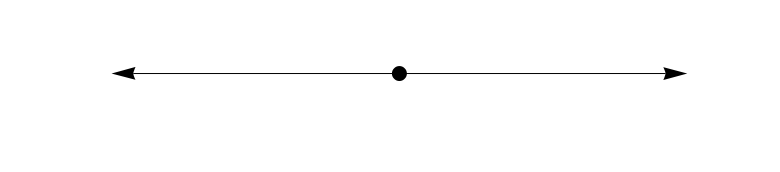
\includegraphics[scale=0.4]{A1.png}
    \caption{Root System $A_1$}
\end{figure}

\begin{namedtheorem}{Classification of Rank 2 Root Systems}
    There exist only 4 reduced, crystallographic root systems (upto isomorphism). Namely,
    \begin{equation*}
    \begin{aligned}
        A_1 \times A_1 &:= \{\pm \alpha_1, \pm \alpha_2 \} \\
        A_2 &:= \{\pm \alpha_1, \pm \alpha_2, \pm (\alpha_1 + \alpha_2) \} \\
        B_2 &:= \{\pm \alpha_1, \pm \alpha_2, \pm (\alpha_1 + \alpha_2), \pm (2 \alpha_1 + \alpha_2) \} \\
        G_2 &:= \{
            \pm \alpha_1,
            \pm \alpha_2,
            \pm (\alpha_1 + \alpha_2),
            \pm (3\alpha_1 + 2\alpha_2),
            \pm (2\alpha_1 + \alpha_2),
            \pm (3\alpha_1 + \alpha_2)
        \}
    \end{aligned}
    \end{equation*}
    where $\alpha_1$ and $\alpha_2$ are roots satisfying the condition that $\|\alpha_1\| \leq \|\alpha\|$ for all $\alpha$ in
    the root system under the induced norm (i.e. $\alpha_1$ is the shortest root) and the angle between $\alpha_1$ and $\alpha_2$,
    $\theta_{\alpha_1, \alpha_2}$ is no smaller than $\pi / 2$.
\end{namedtheorem}

\begin{proof}
    Notice that the roots must span the space $\mathbb{R}^2$. Hence, there must be atleast two linearly independent roots.
    Pick $\alpha_1$ to be the shortest root (under the inner product), i.e. $\|\alpha_1\| \leq \|\alpha\|$ for all 
    $\alpha \in \mathbb{R}^2$. \newline
    
    Choose $\alpha_2$ such that the angle between the two chosen roots is no smaller than $\pi / 2$.
    This is always possible, since if the angle were to be smaller than $\pi / 2$ then $-\alpha_2$, which must also be a root by (R2),
    would have an angle no smaller than $\pi/2$ with $\alpha_1$. \newline
    
    Then Table 1.1 enumerates all possible angles between these roots and given the constraints we deduce that there are only four
    possible cases. We begin with the linearly independent vectors $\alpha_1$ \& $\alpha_2$ and construct from them a root system
    with the four possible cases of angles between them. \newline

    \textbf{Case 1.} $\theta_{\alpha_1, \alpha_2} = \pi / 2$.
    In this scenario, the set $A_1 \times A_1$ is already a root system and any further additions would make it a
    non-reduced root-system. \newline

    \textbf{Case 2.} $\theta_{\alpha_1, \alpha_2} = 2\pi / 3$.
    In this case, we begin with the set $\{\pm \alpha_1, \pm \alpha_2 \}$ and observe that it is not closed under reflection
    through the hyperplane othogonal to its roots.
    It is evident that upon the addition of the element $\pm (\alpha_1 + \alpha_2)$ into the above set, we do get a
    closed root system. \newline

    \textbf{Case 3.} $\theta_{\alpha_1, \alpha_2} = 3\pi / 4$.
    Yet again, begin with the set $\{\pm \alpha_1, \pm \alpha_2 \}$. Computing $\sigma_{\alpha_2}(\alpha_1)$ returns 
    $\alpha_1 + \alpha_2$, and $\sigma_{\alpha_2}(\alpha_1)$ gives $2\alpha_1 + \alpha_2$. Thus adding those into our set
    and performing a final closure check leads to the root system $B_2$. \newline

    \textbf{Case 4.} $\theta_{\alpha_1, \alpha_2} = 5\pi / 6$.
    We repeat the process again, and arrive at 
        $\sigma_{\alpha_2}(\alpha_1) = 3\alpha_1 + \alpha_2$,
        $\sigma_{\alpha_1}(\alpha_1 + \alpha_2) = 2 \alpha_1 + \alpha_2$,
        $\sigma_{\alpha_2}(3 \alpha_1 + \alpha_2) = 3 \alpha_1 + 2 \alpha_2$.
    Thus we obtain our final root system $G_2$.
\end{proof}
\end{document}

\title{Classification of Root Systems}
\author{Shaheer Ziya}

\begin{document}
\maketitle
% In this file you should put the actual content of the blueprint.
% It will be used both by the web and the print version.
% It should *not* include the \begin{document}
%
% If you want to split the blueprint content into several files then
% the current file can be a simple sequence of \input. Otherwise It
% can start with a \section or \chapter for instance.


\chapter{Root Systems}
\section{Defining Root Systems}

\begin{nameddefinition}{Root System}
    Let $E$ be a finite-dimensional Euclidean space with an inner product $\langle \cdot, \cdot \rangle$. \newline
    
    A \textbf{root system} in $E$ is a tuple (E, $\Phi$), where $\Phi$ is a finite, non-empty set of non-zero vectors (called
    \textbf{roots}) satisfying the following properties:
    
    \begin{enumerate}[label=(R{\arabic*})]
        \item $\Phi$ spans $E$.
        \item For every root $\alpha \in \Phi$, the set $\Phi$ is closed under reflection through the hyperplane orthogonal to $\alpha$.
        That is, for any two roots $\alpha, \beta \in \Phi$, the set $\Phi$ contains the element
        \begin{equation*}
            \sigma_\alpha(\beta) = \beta - 2 \ \text{proj}_{\alpha}(\beta).
        \end{equation*}
        where $\text{proj}_{\alpha}(\beta)$ is the projection of $\beta$ on $\alpha$ as shown below.
        \begin{equation*}
            \text{proj}_{\alpha}(\beta) := \frac{ \langle \alpha, \beta \rangle}{\langle \alpha, \alpha \rangle} \alpha
        \end{equation*}
    \end{enumerate}

    The \textbf{rank} of the root system is the dimension of the Euclidean space $E$.
\end{nameddefinition}

For convenience and in contexts where the inner product space is clear, the root system is often referred to simply as $\Phi$.

\begin{example}
    $R_0 = \{\pm \alpha\}$, where $\alpha$ is any fixed non-zero real number, constitutes a root system in $\mathbb{R}$.
\end{example}

\begin{nameddefinition}{Reduced Root System}
    If a root system satisfies the condition that the only multiples of a root, $\alpha$, that are in the root system
    are $\pm \alpha$, then the root system is said to be \textbf{reduced}.
\end{nameddefinition}

\begin{nameddefinition}{Crystallographic Root System}
    If a root system satisfies the integrality condition below, then it is said to be \textbf{crystallographic}.
    \begin{equation*}
        \langle \langle \beta, \alpha \rangle \rangle = 2 \frac{ \langle \alpha, \beta \rangle}{\langle \alpha, \alpha \rangle}
        \in \mathbb{Z} \ \text{for all} \ \alpha, \beta \in \Phi
    \end{equation*}
\end{nameddefinition}

Throughout this text, denote $e_i$ as the $i$-th standard basis vector in $\mathbb{R}^n$.
Then, in combinations such as $\pm e_i \pm e_j$, the signs may be chosen independently.

\begin{example}
    The set $R_1$, shown below, is a root system in $\mathbb{R}^2$ that is neither reduced nor crystallographic.
    \begin{equation*}
        R_1 = \{
            \pm e_1, (\pm \frac{\sqrt{3}}{2}, \pm \frac{1}{2}), (\pm \sqrt{3}, \pm 1) 
        \} 
    \end{equation*}
    $R_1$ spans $\mathbb{R}^2$ and is closed under reflection through the hyperplane orthogonal to any root,
    hence it is a root system.
    
    However, is is not a \textbf{reduced} root system since a scalar multiple of an element in $R_1$,
    namely $2 \cdot (\pm \frac{1}{2}, \pm \frac{\sqrt{3}}{2})$, is contained in $R_1$ itself. 
    It is also not a \textbf{crystallographic} root system because 
    $\langle \langle e_1, (\pm \frac{\sqrt{3}}{2}, \pm \frac{1}{2}) \rangle \rangle = \frac{\sqrt{3}}{2} \notin \mathbb{Z}$.
\end{example}

\begin{example}
    If we remove the redundant multiple in $R_1$ above, we obtain a reduced, non-crystallographic root system $R_2$.
    \begin{equation*}
        R_2 = \{
            \pm e_1, (\pm \frac{\sqrt{3}}{2}, \pm \frac{1}{2})
        \} 
    \end{equation*}
\end{example}

One can also construct examples of non-reduced crystallographic root systems. Consider the following example,

\begin{example}
    The set $R_3$ is a root system in $\mathbb{R}^2$ that is crystallographic but not reduced.
    
    \begin{equation*}
        R_3 = \{
            \pm e_1, \pm e_2, \pm 2 e_1
        \} 
    \end{equation*}
    $R_3$ spans $\mathbb{R}^2$ and is closed under reflection through the hyperplane orthogonal to any root,
    hence it is a root system.
    It is a \textbf{crystallographic} root system because
    $\langle \langle k e_1, e_2 \rangle \rangle = 0$ and $\langle \langle k e_1, k' e_1 \rangle \rangle = kk' \in \mathbb{Z}$,
    where $k,k \in \{\pm 1, \pm 2\}$.
    However, is is not a \textbf{reduced} root system since $2 e_1 \in R_3$.
\end{example}


\begin{example}
    The set $R_4$ is a root system in $\mathbb{R}^2$ that is reduced and crystallographic.
    \begin{equation*}
        R_4 = \{
            \pm e_1, \pm e_2
            \} 
    \end{equation*}
\end{example}

Therefore, we see that a root system may be reduced, crystallographic, both, or neither. \newline

It should be noted that for crystallographic root systems, the integrality condition implies the second condtion (R2)
in root systems since $\sigma_{\alpha}(\alpha) = -\alpha$.
The integrality condition can be interpretted geometerically as follows--the projection of $\beta$ on $\alpha$ is
an integer or half-integer multiple of $\alpha$ since,

\begin{equation*}
    \text{proj}_{\alpha}(\beta) = \frac{1}{2} \langle \langle \beta, \alpha \rangle \rangle \alpha
\end{equation*}

In fact, this is the most restrictive condition since,
\begin{equation*}
    \langle \langle \beta, \alpha \rangle \rangle 
    =  2 \frac{ \langle \alpha, \beta \rangle}{\langle \alpha, \alpha \rangle}
    = 2 \frac{\|\beta\| \|\alpha\| \cos\theta }{\|\alpha\|^2}
    = 2 \frac{\|\beta\|}{\|\alpha\|} \in \mathbb{Z},
\end{equation*}
where $\theta$ is the angle between $\alpha$ and $\beta$.

Furthermore, since $\langle \langle \beta, \alpha \rangle \rangle$ and $\langle \langle \alpha, \beta \rangle \rangle$
must be integers,

\begin{equation*}
    \langle \langle \beta, \alpha \rangle \rangle \cdot \langle \langle \alpha, \beta \rangle \rangle = 4 \cos^2 \theta \in \mathbb{Z}
\end{equation*}

We restate this result as the following lemma.
\begin{lemma}
    For any two roots $\alpha, \beta \in \Phi$, the product
    $\langle \langle \beta, \alpha \rangle \rangle \cdot \langle \langle \alpha, \beta \rangle \rangle$ is an integer.
    More precisely, $4 \cos^2 \theta \in \{ 0, 1, 2, 3, 4 \}.$
    If $4 \cos^2 \theta = 4$, then $\theta = 0$ or $\pi$ and $\beta = \pm \alpha$ which is exactly condition $(R2)$ for a root system.
\end{lemma}

The possible values for $4 \cos^2 \theta$ and the corresponding angles between the roots are displayed in the table below.

\begin{table}[h]
\label{table:enum}
\begin{center}
\begin{tabular}{|| c  c  c  c  c ||}
    \hline $4\cos^2\theta$
&   $\langle \langle \alpha, \beta \rangle \rangle$
&   $\langle \langle \beta, \alpha \rangle \rangle$
&   $\|\alpha\| / \|\beta\|$
&   $\theta$ \\ \hline \hline
    0 & 0 & 0 & N/A & $\pi/2$ \\ \hline
    
    1 & 1 & 1 & 1 & $\pi/3$ \\
      & -1 & -1 & 1 & $2\pi/3$ \\ \hline
    
    2 & 1 & 2 & $\sqrt{2}$ & $\pi/4$  \\
      & -1 & -2 & $\sqrt{2}$ & $3\pi/4$ \\ \hline
    
    3 & 1 & 3 & $\sqrt{3}$ & $\pi/6$ \\
      &-1 & -3 & $\sqrt{3}$ & $5\pi/6$ \\ \hline
\end{tabular}
\end{center}
\caption{The possible angles between roots where, without loss of generality,
the root $\alpha$ is no longer than the root $\beta$ under the induced norm in $E$.
A computation also reveals that $|\langle \beta, \alpha \rangle| \geq |\langle \alpha, \beta \rangle|$.}
\end{table}

Since we aim to classify all root systems, upto isomorhism, it is important to understand when two root systems are
isomorphic. \newline

\begin{nameddefinition}{Root System Isomorphism}
    Two root systems $(E, \Phi)$ and $(F,\Psi)$ are said to be isomorphic if there exists a linear isomorphism
    $\varphi: E \to F$ such that $\varphi(\Phi) = \Psi$
    and preserves the number $\langle \langle x, y \rangle \rangle$ for each pair of roots.
\end{nameddefinition}

\begin{example}
    The root systems $R = \{ \pm e_1, \pm e_2 \} $ and $R' = \{ \pm e_1 \pm e_2 \}$ are isomorphic.
\end{example}

\begin{example}
    The root systems
    $S = \{ \pm e_1, \pm e_2, \pm e_1 \pm e_2 \} $ and
    $S' = \{ \pm e_1, (\pm \frac{\sqrt{3}}{2}, \pm \frac{1}{2}) \}$ are not isomorphic.
\end{example}

Finally, we wish to exclude root systems that can be constructed from direct sums of smaller root systems.
This motivates the following definition. \newline

\begin{nameddefinition}{Decomposable Root System}
    A Root System $\Phi$ is said to be \textbf{decomposable} if there is a proper decomposition
    $\Phi = \Phi_1 \cup \Phi_2$ such that $\Phi_1$ and $\Phi_2$ are root systems in $E$ and $\Phi_1 \perp \Phi_2$ (i.e. 
    $\forall \alpha_1 \in \Phi_1 , \forall \alpha_2 \in \Phi_2,  \langle \alpha_1, \alpha_2 \rangle = 0$). \newline 

    Otherwise, $\Phi$ is said to be \textbf{indecomposable}. 
    Often, in literature, such root systems are also called \textbf{irreducible}.
    We adopt the term indecomposable to avoid confusion with the notion of reduced root systems.
\end{nameddefinition}

\begin{example}
    The root system $R_4 = \{ \pm e_1, \pm e_2 \}$ is an indecomposable, reduced, crystallographic root system.
\end{example}

\begin{example}
    The root system $R_5 = \{ \pm e_1, \pm e_2 \} \cup \{ \pm 2 e_1 \}$ is a decomposable root system.
\end{example}

This report concerns itself primarily with reduced, crystallographic root systems, simply referred to as root systems henceforth,
unless otherwise specified.

\footnote{
    The provided definition differs from the more general definition stated in Lean 4's MathLib.
    In Lean 4, root systems are defined over modules instead of Euclidean spaces among other minor differences.
    As such, when neccessary the proofs in Lean 4 restrict the more general definition to our definition.
    Of note, root systems in Lean 4 are assumed to be reduced, crystallographic root systems.} \newline

    \section{Classifying Root Systems of Small Rank}

% Classification of Rank 1 Root Systems
\begin{namedtheorem}{Classification of Rank 1 Root Systems}
    The only indecomposable, reduced, crystallographic root systems of rank 1 (upto isomorhism) is $A_1 = \{ \pm \alpha \}$ [See Figure 1.1], where $\alpha$ is any fixed non-zero real number.
\end{namedtheorem}

\begin{proof}
    Let $\Phi$ be a reduced, crystallographic root system of rank 1.
    Let $\alpha \in \Phi$ be a non-zero root.
    Since $\Phi$ is reduced, the only multiples of $\alpha$ in $\Phi$ are $\pm \alpha$.
    Therefore, $\Phi = \{ \pm \alpha \}$.
    Clearly, if the root system depends on $\alpha$ where $\Phi_{\alpha} = \{ \pm \alpha \}$,
    then for any non-zero $\alpha_1, \alpha_2$ in the Euclidean space, $\Phi_{\alpha_1}$ is isomorphic
    to $\Phi_{\alpha_2}$.
\end{proof}

\begin{figure}[h]
    \centering
    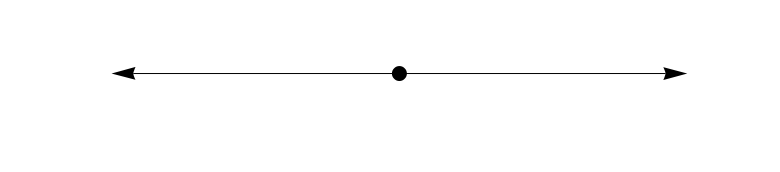
\includegraphics[scale=0.4]{A1.png}
    \caption{Root System $A_1$}
\end{figure}

\begin{namedtheorem}{Classification of Rank 2 Root Systems}
    There exist only 4 reduced, crystallographic root systems (upto isomorphism). Namely,
    \begin{equation*}
    \begin{aligned}
        A_1 \times A_1 &:= \{\pm \alpha_1, \pm \alpha_2 \} \\
        A_2 &:= \{\pm \alpha_1, \pm \alpha_2, \pm (\alpha_1 + \alpha_2) \} \\
        B_2 &:= \{\pm \alpha_1, \pm \alpha_2, \pm (\alpha_1 + \alpha_2), \pm (2 \alpha_1 + \alpha_2) \} \\
        G_2 &:= \{
            \pm \alpha_1,
            \pm \alpha_2,
            \pm (\alpha_1 + \alpha_2),
            \pm (3\alpha_1 + 2\alpha_2),
            \pm (2\alpha_1 + \alpha_2),
            \pm (3\alpha_1 + \alpha_2)
        \}
    \end{aligned}
    \end{equation*}
    where $\alpha_1$ and $\alpha_2$ are roots satisfying the condition that $\|\alpha_1\| \leq \|\alpha\|$ for all $\alpha$ in
    the root system under the induced norm (i.e. $\alpha_1$ is the shortest root) and the angle between $\alpha_1$ and $\alpha_2$,
    $\theta_{\alpha_1, \alpha_2}$ is no smaller than $\pi / 2$.
\end{namedtheorem}

\begin{proof}
    Notice that the roots must span the space $\mathbb{R}^2$. Hence, there must be atleast two linearly independent roots.
    Pick $\alpha_1$ to be the shortest root (under the inner product), i.e. $\|\alpha_1\| \leq \|\alpha\|$ for all 
    $\alpha \in \mathbb{R}^2$. \newline
    
    Choose $\alpha_2$ such that the angle between the two chosen roots is no smaller than $\pi / 2$.
    This is always possible, since if the angle were to be smaller than $\pi / 2$ then $-\alpha_2$, which must also be a root by (R2),
    would have an angle no smaller than $\pi/2$ with $\alpha_1$. \newline
    
    Then Table 1.1 enumerates all possible angles between these roots and given the constraints we deduce that there are only four
    possible cases. We begin with the linearly independent vectors $\alpha_1$ \& $\alpha_2$ and construct from them a root system
    with the four possible cases of angles between them. \newline

    \textbf{Case 1.} $\theta_{\alpha_1, \alpha_2} = \pi / 2$.
    In this scenario, the set $A_1 \times A_1$ is already a root system and any further additions would make it a
    non-reduced root-system. \newline

    \textbf{Case 2.} $\theta_{\alpha_1, \alpha_2} = 2\pi / 3$.
    In this case, we begin with the set $\{\pm \alpha_1, \pm \alpha_2 \}$ and observe that it is not closed under reflection
    through the hyperplane othogonal to its roots.
    It is evident that upon the addition of the element $\pm (\alpha_1 + \alpha_2)$ into the above set, we do get a
    closed root system. \newline

    \textbf{Case 3.} $\theta_{\alpha_1, \alpha_2} = 3\pi / 4$.
    Yet again, begin with the set $\{\pm \alpha_1, \pm \alpha_2 \}$. Computing $\sigma_{\alpha_2}(\alpha_1)$ returns 
    $\alpha_1 + \alpha_2$, and $\sigma_{\alpha_2}(\alpha_1)$ gives $2\alpha_1 + \alpha_2$. Thus adding those into our set
    and performing a final closure check leads to the root system $B_2$. \newline

    \textbf{Case 4.} $\theta_{\alpha_1, \alpha_2} = 5\pi / 6$.
    We repeat the process again, and arrive at 
        $\sigma_{\alpha_2}(\alpha_1) = 3\alpha_1 + \alpha_2$,
        $\sigma_{\alpha_1}(\alpha_1 + \alpha_2) = 2 \alpha_1 + \alpha_2$,
        $\sigma_{\alpha_2}(3 \alpha_1 + \alpha_2) = 3 \alpha_1 + 2 \alpha_2$.
    Thus we obtain our final root system $G_2$.
\end{proof}
\end{document}